\section{Implementierung des SmBasicSafeRetries}

Der nächste DEA verwendet den SmBasic als Grundlage und soll das Problem des vorzeitigen Abbruchs verhindern. Dabei sollen keine neuen Inkonsistenzquellen eingeführt werden. 

\subsection{Verhinderung eines Vorzeitigen Abbruchs}

\paragraph*{Netzwerkfehler} \mbox{}\\
Für alle Transaktionen, die nicht zu einer Änderung des Systemzustands eines Teilnehmerservices führen, können Retries im Falle eines Netzwerkfehlers eingeführt werden. Dazu gehören \textit{GetArticleData} und \textit{GetShipmentStatus}. 

\paragraph*{Lastfehler} \mbox{}\\
Behindern sich mehrere parallele lokale Transaktionen innerhalb eines Teilnehmerservices, kommt es zu einer Race Condition (Wettlaufsituation). Dabei gewinnt die erste lokale Transaktion T1 und kann wie gewohnt abgeschlossen werden. Alle lokalen Transaktionen, die innerhalb der Bearbeitungszeit von T1 auf die gesperrten Ressourcen zugreifen, schlagen fehl. Die aus diesem Fehler resultierende Response enthält den Http-Statuscode 429 und wird vom Koordinator auf ein entsprechendes Ergebnis gemappt. Dieses Verhalten ist für den StockService und die BankServices implementiert. 

Antwortet ein Service mit einer solchen Response, ist der Fehler durch einen Retry auflösbar. Das bedeutet, dass für die lokalen Transaktionen \textit{BlockArticles}, \textit{RemoveMoney}, \textit{AddMoney} und \textit{StartShipment} ein Retry eingeführt werden kann. Ebenso kann diese Stategie auf alle zugehörigen Kompensierungen angewendet werden.

\paragraph*{DEA SmBasicSafeRetries} \mbox{}\\
Aus den beschriebenen Anpassungen ergibt sich der SmBasicSafeRetries in \cref{fig:SmBasicSafeRetries}. 

\begin{figure}[h!]
	\centering
	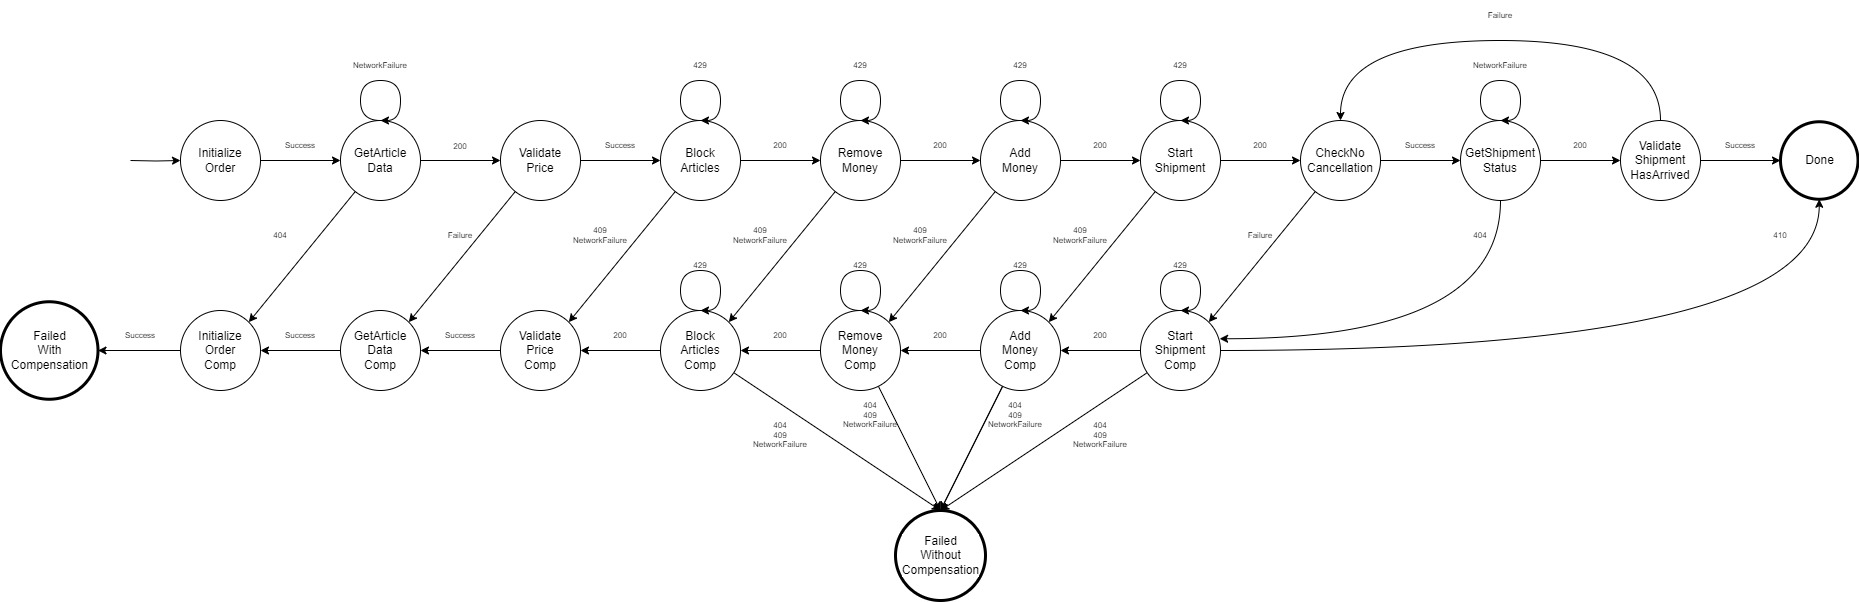
\includegraphics[width=\linewidth]{figures/ChapterVersuchsdurchführung/sm_basic_safe_retries.jpg}
	\caption{DEA für SmBasicSafeRetries}
	\label{fig:SmBasicSafeRetries}
\end{figure}
\FloatBarrier

\subsection{StateAnalysisResult}

Das StateAnalysisResult von SmBasicSafeRetries und SmBasic sind wie erwartet sehr ähnlich. Im Testfall FinishOrders ist zu sehen, dass die Werte für \textit{isSuccessFullTestInstancePercentage} deutlich höher sind. Die vorzeitigen Abbrüche aufgrund von Last- und Netzwerkfehlern an unkritischen nicht-transaktionellen Stellen wurden durch das Einführen von Retries eliminiert. In Testszenario 1 führt dies dazu, dass 100\% der Sagas erfolgreich sind. Das gilt auch für den Testfall CancelOrders.

\paragraph*{Testfall FinishOrders} \mbox{}\\
\begin{center}
	\fontsize{9}{12}\selectfont
	\begin{longtable}[h]{|p{5cm}|p{1cm}|p{1cm}|p{1cm}|}
		\hline
		Messwert & S1 & S2 & S3 \\ \hline
		\endhead
		%\label{tab:smbasicsaferetries_stateanalysisresult_finishorders}
		\endfoot
		successfull\-Percentage & 1.0 & 0.65 & 0.39 \\ \hline
		finished\-Percentage & 1.0 & 1.0 & 1.0 \\ \hline
		pending\-Percentage & 0.0 & 0.0 & 0.0 \\ \hline
		failedWithCompensation\-Percentage & 0.0 & 0.31 & 0.47 \\ \hline
		failedWithoutCompensation\-Percentage & 0.0 & 0.05 & 0.15 \\ \hline
		hasCorrectEndstate\-Percentage & 1.0 & 0.65 & 0.39 \\ \hline
		containsAllExpectedLogs\-Percentage & 1.0 & 0.65 & 0.39 \\ \hline
		isSuccessfullTestInstance\-Percentage & 1.0 & 0.65 & 0.39 \\ \hline
	\end{longtable}
\end{center}
\FloatBarrier

\paragraph*{Testfall CancelOrders} \mbox{}\\
\begin{center}
	\fontsize{9}{12}\selectfont
	\begin{longtable}[h]{|p{5cm}|p{1cm}|p{1cm}|p{1cm}|}
		\hline
		Messwert & S1 & S2 & S3 \\ \hline
		\endhead
		%\label{tab:smbasicsaferetries_stateanalysisresult_cancelorders}
		\endfoot
		successfull\-Percentage & 0.0 & 0.0 & 0.0 \\ \hline
		finished\-Percentage & 1.0 & 1.0 & 1.0 \\ \hline
		pending\-Percentage & 0.0 & 0.0 & 0.0 \\ \hline
		failedWithCompensation\-Percentage & 1.0 & 0.77 & 0.64 \\ \hline
		failedWithoutCompensation\-Percentage & 0.0 & 0.24 & 0.37 \\ \hline
		hasCorrectEndstate\-Percentage & 1.0 & 0.77 & 0.64 \\ \hline
		containsAllExpectedLogs\-Percentage & 1.0 & 0.47 & 0.17 \\ \hline
		isSuccessfullTestInstance\-Percentage & 1.0 & 0.47 & 0.17 \\ \hline
	\end{longtable}
\end{center}
\FloatBarrier

\subsection{TransactionAnalysisResult}
Das TransactionAnalysisResult zeigt, dass der Messwert \textit{consistentSagasPercentage} im Vergleich zu SmBasic sinkt. Das ist damit zu erklären, dass die vorzeitigen Abbrüche im SmBasic das Ergebnis deutlich maskiert haben. Durch die vorzeitigen Abbrüche im SmBasic war die Gesamtzahl an Transaktionen niedriger. Das bedeutet, dass es weniger Möglichkeiten gab, einen Fehler zu verursachen, der zu Inkonsistenz führt.

Die Inkonsistenz ist bei dem Testfall für CancelOrders niedriger als bei FinishOrders. Das hat denselben Grund, der Testfall CancelOrders durchläuft zusätzlich zu den Ts immer die zugehörigen Cs und kann somit in häufigeren Zuständen Inkonsistenzen verursachen.

\begin{center}
	\fontsize{9}{12}\selectfont
	\begin{longtable}[h]{|p{5cm}|p{1cm}|p{1cm}|p{1cm}|}
		\hline
		& S1 & S2 & S3 \\ \hline
		\endhead
		%\label{tab:smbasic_stateanalysisresult}
		\endfoot
		FinishOrders & 1 & 1 & 0.74\\ \hline	
		CancelOrders & 1 & 1 & 0.54\\ \hline
	\end{longtable}
\end{center}
\FloatBarrier